\documentclass[11pt]{article}
\usepackage[T1]{fontenc}
\usepackage[utf8]{inputenc}
\usepackage[right=2.5cm, left=2.5cm, bottom=4cm, top=3cm]{geometry}
\usepackage[french]{babel}
\usepackage{textcomp}
\usepackage{graphicx}
\usepackage{mathtools,amssymb,amsthm}
\usepackage{lmodern}
\usepackage{multirow}
\usepackage{array}
\usepackage{algorithm}
\usepackage{algorithmic}

\title{\vspace{13em}{\huge TER}}
\author{Rémi Navarro - 21401257\\ Edouard Fouassier - 21400750}

\begin{document}

\pagenumbering{gobble}
\clearpage
\maketitle\vspace{13em}
\newpage
\tableofcontents
\newpage
\clearpage
\pagenumbering{arabic}

\section{Introdution}
Dans le cadre du module TER du S2 Master Informatique à l’UVSQ, nous avons eu l’occasion de réaliser un projet sous la direction de Mr Yann Strozecki et Mael Guiraud.
Nous avons choisi, parmi les sujets proposés, le sujet "Algorithme glouton de remplissage" car c'est un sujet qui demande une bonne compréhension de l'algorithmique ce qui nous a beaucoup intéressé.

De nos jours les échanges par les différents réseaux sont centralisés dans des datacenters ou cloud.
Pour gagner en efficacité il faut minimisé la latence lors de l'envoie d'un message vers un cloud.

L'objectif de ce projet est de concevoir et comparer des algorithmes gloutons qui permettent de placer au mieux des tâches periodiques avec des contraintes portant sur les paires de tâches.
Pour cela nous utilisons un modèle où les tâches sont envoyées periodiquement et le temps entre l'envoie et la reception est fixe.
Dans ce modèle il y a deux périodes de taille P, l'envoie d'une tâches est placé sur la première période et la réception sur la seconde après un delai.
Il faut donc réussir à placer un maximum de tâches dans la période.

\section{Structures de données}

Dans un premier temps nous utilisions les structures suivantes :\\\\
Une structure "Task" représentant les tâches, composées de 3 entiers : le numero de la tâche, son délai et sa place qui est initialisé a -1, ainsi qu'un tableau de deux entiers, un pour le cycle aller et un pour le cycle retour.\\ 
\\\\
Les taches "Task" étaient liées avec la structure chaine.\\\\
\indent \textbf{Chaine} \{ \\
    \indent \indent Task t   \indent \indent \indent //une tache\\
    \indent \indent chaine $\uparrow$next \indent //la tache suivante.\\
\indent\}
\\\\
\indent La période était stockée dans deux tableaux d'entier, nous écrivions le numéro de la tâche dans la ou les case(s) qu'elle occupait.\\
Mais comme seul les espaces disponibles de la periode nous interesse, cette structure n'était pas optimale.\\
Nous sommes donc passé à une structure représentant les espaces libres de la periode sous forme d'une chaine.
\begin{center}
    \begin{tabular}{|l|c|c|}			
    \hline                                              & \textbf{Structure initiale}   & \textbf{Nouvelle structure} \\
    \hline 	Periode initiale de taille 10               & [0,0,0,0,0,0,0,0,0,0]         &(0,9)		     \\
    \hline 	Placement d'une tache de taille de en 5 	& [0,0,0,0,0,1,1,0,0,0] 		& (0,4)$\rightarrow$(6,9)   \\
    \hline
    \end{tabular}\vspace{1em}
\end{center}
\noindent Les taches n'étant plus stockées dans une liste mais dans un tableau, cela a permis de réduire la mémoire utilisée et d'augmenter la taille des tests effectués.\\\\
La structure Periode est utilisée pour représenter les intervalles disponibles d'une période.\\\\
\indent \textbf{Periode} \{ \\
    \indent \indent entier begin    \indent \indent//Le debut de la periode libre\\
    \indent \indent entier end \indent \indent //La fin de la periode libre.\\
    \indent \indent Periode $\uparrow$next \indent //La periode libre suivante.\\
\indent\}
\\\\
La structure Tasktab représente un tableau de tâches.\\\\
\indent \textbf{Tasktab} \{ \\
    \indent \indent Task tab    \indent \indent//Le debut de la periode libre\\
    \indent \indent entier taille \indent   //La fin de la periode libre.\\
\indent\}

\section{Algorithmes}

L'algorithme "FirstFit" place dans la période les tâches par ordre d'arrivée, au premier endroit disponible (first fit), si la tâche ne peut pas être placée, on passe à la suivante.
\begin{algorithm}
    \caption{FirstFit}
    \begin{algorithmic}
    \REQUIRE Tasktab, PeriodeMax
    \FOR{chaque Task dans Tasktab}
        \FOR {$i \leftarrow  0$ to PeriodeMax}
         \IF {task entre dans la periode aller et t entre dans la periode retour après le delay}
            \STATE $task.place \leftarrow i$
         \ENDIF
        \ENDFOR
    \ENDFOR
    \RETURN Tasktab
    \end{algorithmic}
\end{algorithm}

C'est l'algorithme le plus trivial, il a une complexité faible en O(n*m) avec n le nombre de tâches et m la taille de la période.\\
Un exemple de placement des tâches est fourni en Annexe (cf Figure 1)\\

\newpage
L'algorithme "AlgoLourd" calcul pour chaques tâches son nombre de places disponibles puis place celle ayant le plus de contraintes.\\
\begin{algorithm}
    \caption{AlgoLourd}
    \begin{algorithmic}
    \REQUIRE Tasktab, PeriodeMax
    \STATE $min \leftarrow PeriodeMax$
    \STATE $taskMin \leftarrow 0$
    \STATE $libreMin \leftarrow 0$
    \FOR{chaque Task}
        \FOR {chaque Task t dans Tasktab}
        \STATE $compteur \leftarrow 0$
        \STATE $libre \leftarrow 0$
            \FOR {$i \leftarrow  0$ to PeriodeMax}
                \IF {t entre dans la periode aller et t entre dans la periode retour après le delay}
                    \STATE $compteur \leftarrow compteur + 1$
                    \STATE $libre \leftarrow i$
                \ENDIF
            \ENDFOR
            \IF {compteur <= compteurMin}
                \STATE $compteur \leftarrow compteurMin$
                \STATE $taskMin \leftarrow t$
                \STATE $libreMin \leftarrow libre$
            \ENDIF
        \ENDFOR
        \STATE $taskMin.place \leftarrow libreMin$
    \ENDFOR
    \RETURN Tasktab
    \end{algorithmic}
\end{algorithm}

C'est l'algorithme qui permet de placer le plus de taches parmi nos quatres algorithmes mais il est 30 fois plus long que l'algorithme "FirstFit".\\
Sa complexité est O($n^2*m$) avec n le nombre de tâches et m la taille de la période.\\ 
Un exemple de placement des tâches est fourni en Annexe (cf Figure 2)\\

\newpage
L'algorithme "AlgoSuperLourd" calcul pour chaques tâches celle qui bloque le plus les autres et on place en priorité les moins contraignantes.\\
\begin{algorithm}
    \caption{AlgoSuperLourd}
    \begin{algorithmic}
    \REQUIRE Tasktab, PeriodeMax
    \STATE $cptAvant[tasktab.nbTask]$
    \STATE $gene[tasktab.nbTask]$
    \FOR{chaque Task}
        \STATE $cptAvant[] \leftarrow cptplace()$ (cptplace() permet de compter le nombre de places disponibles pour chaque tâche)
        \STATE $cptApres[tasktab.nbTask]$
        \FOR {chaque Task t dans Tasktab}
            \STATE $gene[t] \leftarrow 0$
            \FOR {$i \leftarrow  0$ to PeriodeMax}
                \IF {t entre dans la periode aller et t entre dans la periode retour après le delay}
                    \STATE Place t
                \ENDIF
            \ENDFOR
            \STATE $cptApres[] \leftarrow cptplace()$ //cptplace() permet de compter le nombre de places disponibles pour chaque tâche
            \STATE $gene[t] \leftarrow \sum\limits_{i\leftarrow0}^{Tasktab.nbTask} cptAvant[i] - cptApres[i]$
            \STATE Retire t de la periode
        \ENDFOR
        \STATE Place les Task dans l'ordre croissant de génance
    \ENDFOR
    \RETURN Tasktab
    \end{algorithmic}
\end{algorithm}

Dans cet algorithme on utilise la fonction cptplace() qui a une compléxité O(n*m) qui augmente grandement la compléxité de l'algorithme "AlgoSuperLourd".\\
On obtient donc une complexité O($n^3*m$), avec n le nombre de tâches et m la taille de la période, ce qui le rend bien moins intéressant que les autres, de plus il place moins de taches.\\
Un exemple de placement des tâches est fourni en Annexe (cf Figure 3)\\

\newpage
L'algorithme "AlgoPasilourd" calcul la valeur delay mod(cycle) de chaques tâches, cela permet de les regrouper sur une période et de bien les ordonner sur l'autre.\\
\begin{algorithm}
    \caption{AlgoPasilourd}
    \begin{algorithmic}
    \REQUIRE Tasktab, PeriodeMax, nbTask
    \STATE $val[nbTask]$
    \STATE $cycle$ $\leftarrow$ cycle des tâches
    \FOR{chaque tache t}
        \STATE $tmpval \leftarrow tasktab.tab[t].delay\%cycle$
        \STATE Placement de tmpval dans le tableau val dans l'ordre croissant des tmpval
    \ENDFOR
    \STATE Placement de la tâche t ayant la valeur val[t] la plus grande à l'emplacement $periodeMax - val[t]$ de la période de retour et son correspondant sur la période aller
    \STATE $nbPlace \leftarrow 1$
    \FOR{le nombre de tâches}
        \FOR{chaque tâches t par ordre décroissant de val[t]}
            \IF{Placement de la tâche t de la tâche t ayant la valeur val[t] la plus grande à l'emplacement $periodeMax - val[t] + nbPlace * cycle$ de la période de retour et son correspondant sur la période aller possible}
                \FOR {$i \leftarrow  0$ to PeriodeMax}
                    \IF {task entre dans la periode aller et t entre dans la periode retour après le delay}
                        \STATE $t.place \leftarrow i$
                    \ENDIF
                \ENDFOR
                \STATE $nbPlace \leftarrow nbPlace+1$
            \ENDIF
        \ENDFOR
    \ENDFOR
    \STATE Pour toute les tâches qui n'ont pas été placé, on essaye de les placer à la manière d'un FirstFit
    \RETURN Tasktab
    \end{algorithmic}
\end{algorithm}

C'est un algorithme moyen, il est un peu plus long que l'algorithme "FirstFit" et un peu moins efficace.\\
Sa complexité est O($n^2*m$) avec n le nombre de tâches et m la taille de la période.\\ 
Un exemple de placement des tâches est fourni en Annexe (cf Figure 4)\\

\section{Analyse}
Pour chaques tests effectués les paramètres utilisés sont : période de 50000, cycle de taille 1000 et 100 essais.\\
\\
Nous avons réaliser plusieurs mesures :
\begin{itemize}
    \item celle du taux de réussite, un algorithme reussi lorsqu'il arrive à placer toutes les tâches données. (cf Figure 5 en Annexe)
    \item celle du taux de complétion, le taux de completion d'un algorithme est le pourcentage de tâches qu'il a reussi à mettre parmi les tâches données. Sur ce graphique, la ligne représente le taux de complétion moyen, les points le taux de complétion minimum et les losanges le taux de complétion maximum. (cf Figure 6 en Annexe)
    \item celle du temps moyen. (cf Figure 7 en Annexe)\\
\end{itemize}

 Sur le graphique du taux de reussite (Figure 5) nous pouvons constater que l'algoLourd est le plus efficace.\\
 Il parvient à 100\% de réussite jusqu'à 32 tâches sur les 50 possibles, son taux de réussite d'écroit fortement au-delà.\\
 Le FirstFit est un peu moins efficace, il conserve un taux de réussite de 100\% jusqu'à 28 tâches mais celui decroit doucement puis chute à 32 tâches.\\
 L'algoPasiLourd a une efficacité proche du FirstFit mais légèrement plus faible et il devient totalement inefficace plus vite.\\
 L'algoSuperLourd a une courbe en dessous des autres à partir de 26 tâches.\\

 Sur le graphique suivant (Figure 6) nous pouvons constaté que l'allure est la même.\\
L'algoLourd est le plus efficace et parvient à placer 78\% des tâches quand il y a autant de tâches que de places. Ses taux de complétion minimum et maximum sont les moins extrêmes.\\ 
L'algoSuperLourd est le plus mauvais avec un taux de complétion maximum élevé mais un taux minimum très faible.\\

Le dernier graphe (Figure 7) apporte plus d'information, il représente le temps moyen de chaque algorithme.\\
Nous pouvons voir qu'il y a un algorithme ayant un temps bien supérieur aux autres, l'algoSuperLourd, il est jusqu'à 3000 fois plus long.\\
L'algorithme FirstFit et l'algoPasilourd ont un temps similaire (ligne la plus basse) et l'algoLourd est un peu plus long, 30 fois dans le pire des cas.\\
La différence de temps d'exécution entre les algorithme ayant la même complexité s'explique par la fragmentation de la periode. Certains algorithme génère une periode très fragmenté bien plus longue à parcourir.


\section{Conclusion}

Après ces différentes analyse nous pouvons determiné que, parmis ces algorithmes, si nous voulons placer le plus de tâches l'algoLourd est le plus efficace, il parvient a garder un taux de réussite totale plus longtemps et après cela sont taux de complétion est plus élevé.\\
Si nous voulons un algorithme rapide, le FirstFit est recommandé, il est plus rapide et reste très efficace. Si nous voulons trouver un juste milieu le FirstFit est le meilleur car il est rapide et a une efficacité proche de l'algoLourd.\\

\newpage
\section{Annexes}
% \subsection{Exemples d'exécutions}
Pour chaques exécutions des algorithmes, les paramètres sont :
\begin{itemize}
    \item Nombre de tâches : 10
    \item Cycle aller et retour des taches : 2
    \item Taille de la période : 20
    \item Délai des tâches :
    \begin{itemize}
        \item Tache 0 : 3
        \item Tache 1 : 6
        \item Tache 2 : 17
        \item Tache 3 : 15
        \item Tache 4 : 13
        \item Tache 5 : 15
        \item Tache 6 : 6
        \item Tache 7 : 12
        \item Tache 8 : 9
        \item Tache 9 : 1
    \end{itemize}
\end{itemize}

\begin{figure}[!ht]
    \center
    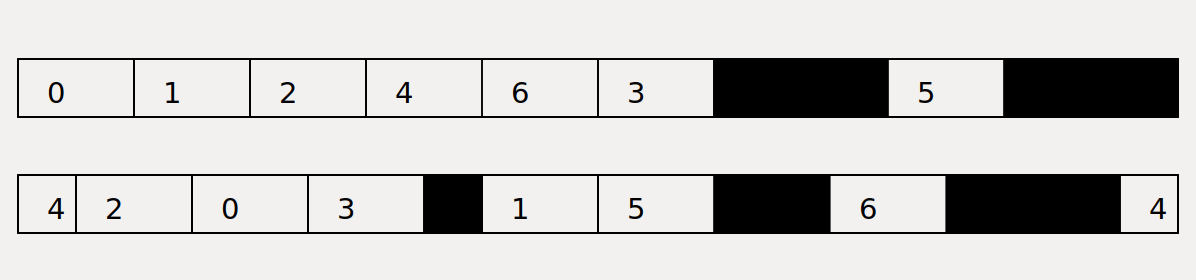
\includegraphics[scale = 0.35]{FirstFit}    
    \caption{Placement des tâches avec l'algorithme "FirstFit"}
\end{figure} 
\begin{figure}[!ht]
    \center
    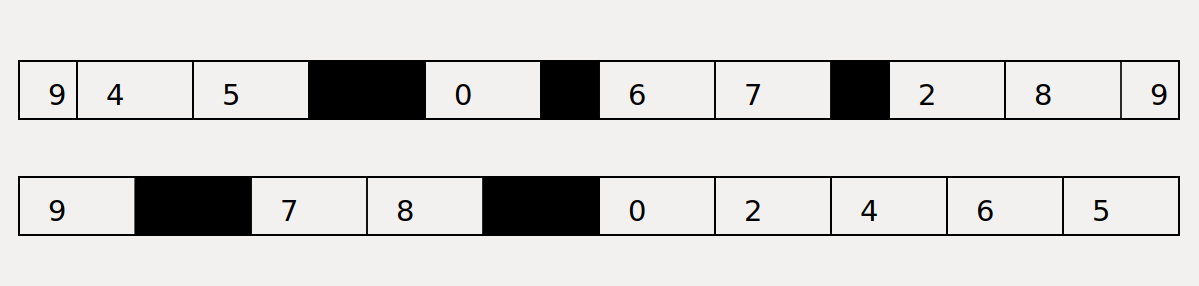
\includegraphics[scale = 0.35]{AlgoLourd}
    \caption{Placement des tâches avec l'algorithme "AlgoLourd"}
\end{figure}
\newpage
\begin{figure}[!ht]
    \center
    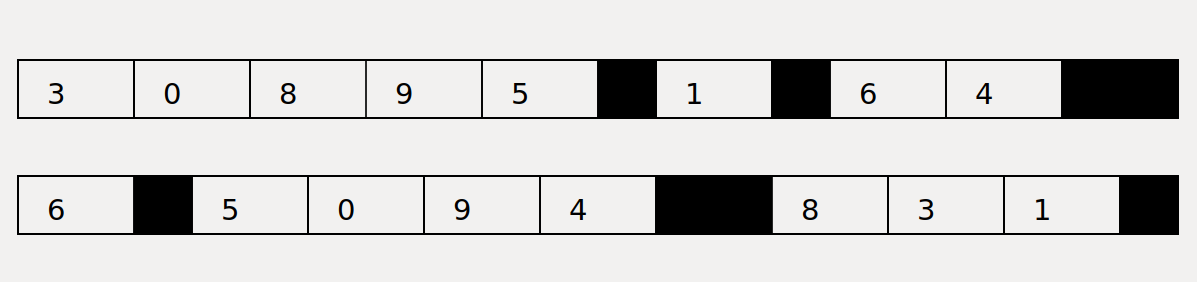
\includegraphics[scale = 0.35]{AlgoSuperLourd}
    \caption{Placement des tâches avec l'algorithme "AlgoSuperLourd"}
\end{figure}
\begin{figure}[!ht]
    \center
    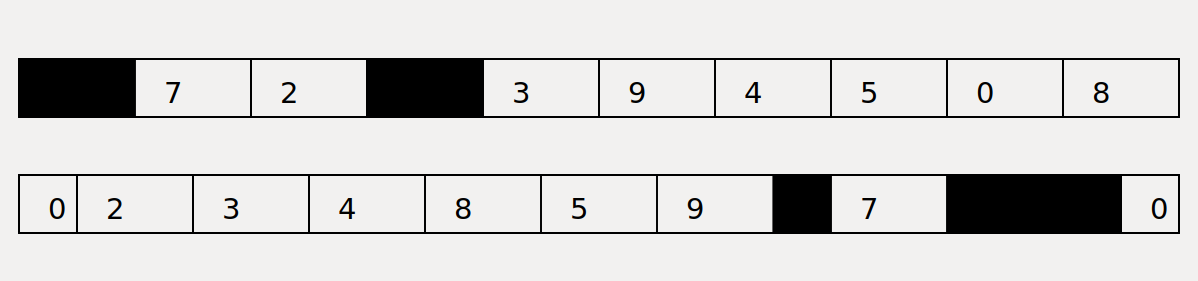
\includegraphics[scale = 0.35]{AlgoPasiLourd}
    \caption{Placement des tâches avec l'algorithme "AlgoPasiLourd"}
\end{figure}


% \subsection{Graphes}
\newpage
Pour chaques graphes les paramètres utilisés sont : période de 50000, cycle de taille 1000 et 100 essais.
\begin{figure}[!ht]
    \center
    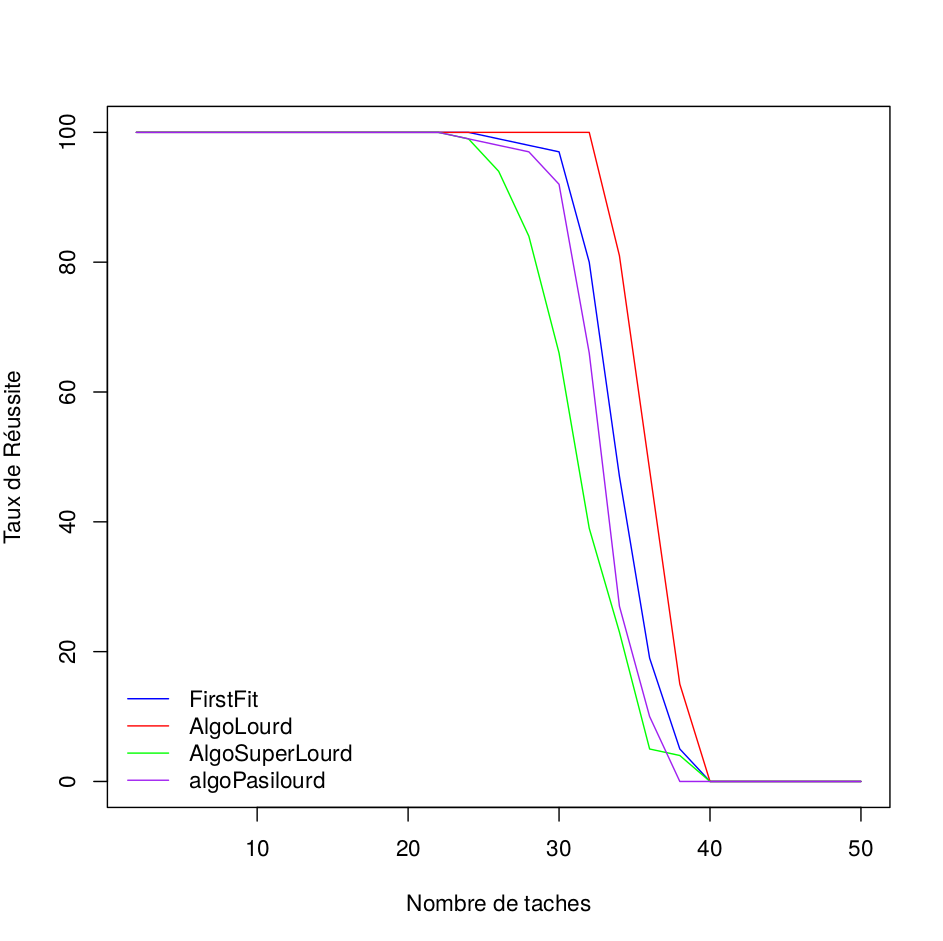
\includegraphics[scale = 0.4]{taux_reussite}
    \caption{Taux de réussite des algorithmes sur 100 essais en fonction du nombre de tâches}
\end{figure} 

\begin{figure}[!ht]
    \center
    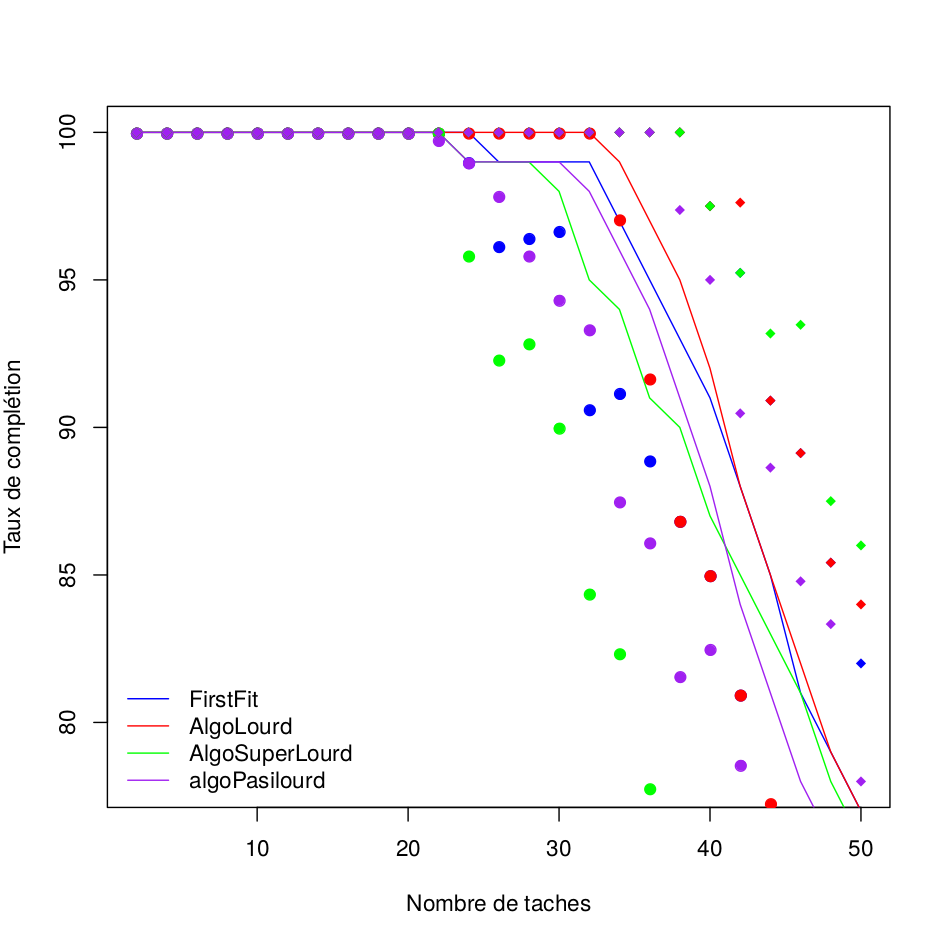
\includegraphics[scale = 0.4]{taux_completion}
    \caption{Taux de complétion des algorithmes sur 100 essais en fonction du nombre de tâches}
\end{figure}

\begin{figure}[!ht]
    \center
    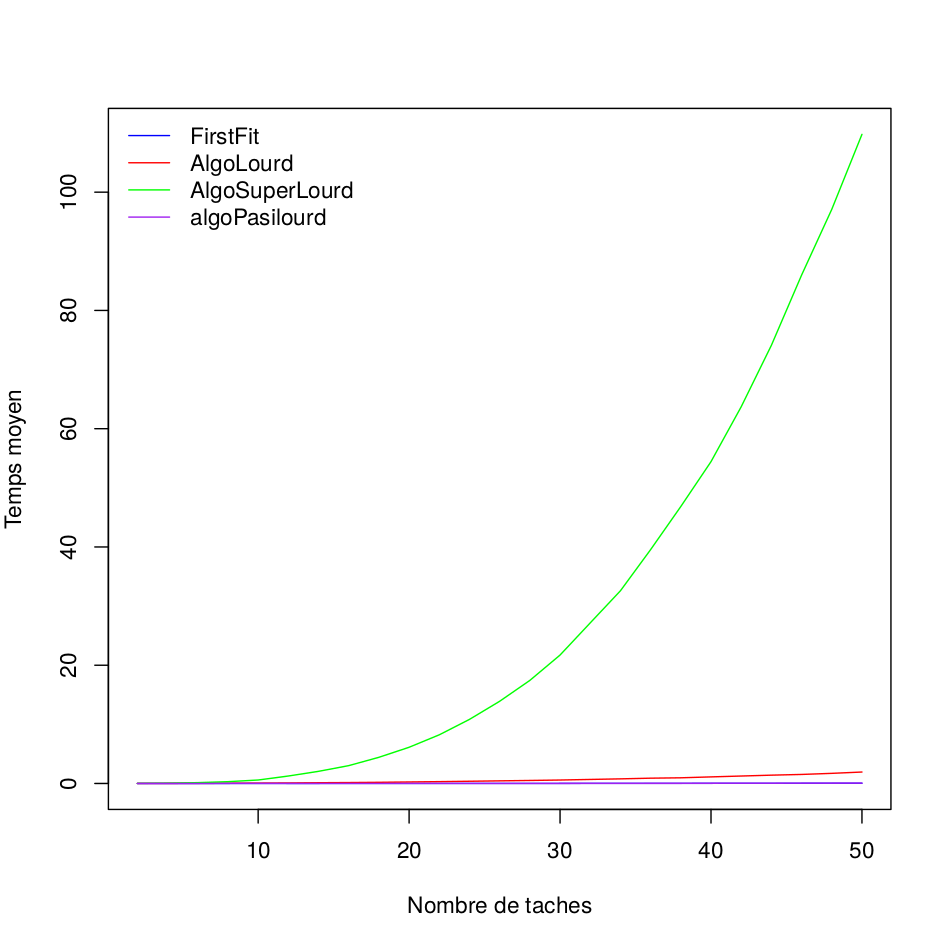
\includegraphics[scale = 0.4]{temps_moyen}
    \caption{Temps moyen d'exécution des algorithmes sur 100 essais en fonction du nombre de tâches}
\end{figure}

\end{document}